% Draft for UIST 2027 (ACM acmart, sigconf). Build: latexmk -pdf main.tex
% Numbers marked \measured{} come from results/ in this repository; \todo{} marks what is not done.
\documentclass[sigconf,review,anonymous]{acmart}
\usepackage{booktabs}
\usepackage{xcolor}
\usepackage{tikz}
\usetikzlibrary{arrows.meta,shapes.geometric}
\newcommand{\todo}[1]{\textcolor{red}{[TODO: #1]}}
\newcommand{\measured}[1]{#1}
\newcommand{\sys}{RoomCall}

\begin{document}

\title{\sys: A Live, Photoreal, Physically Shared Copy of a Real Room for Ordinary Video Calls}

\begin{abstract}
Video calls show faces, not places. When one person wants others to see, and act in, the room
they are in, today's options are a shaky camera tour or a headset-only telepresence system.
We present \sys, which turns a phone LiDAR scan into a room that everyone on an ordinary Zoom,
Meet or Teams call can open from a link in the chat. Everyone walks around in the browser, grabs,
throws and rearranges the real furniture, and opens doors and drawers, with one physics
simulation on a server so that all participants see the same room. The room is built
progressively. A physics-ready sketch appears in \measured{2\,s}, and a photoreal Gaussian-splat
room from the scan's own photos and LiDAR in \measured{10\,s}. A sharper, trained room streams
in over the following \measured{1.5\,min}, while each object's generated mesh and articulation
arrive in the background. To make the photoreal room interactive, we cut every movable object
out of the splat with SAM~2 masks voted onto the splats, move its physics body to where the
photos show it (but never into a wall), and patch the floor that no photo saw. We report build
times and costs, visual fidelity on held-out photos, physics plausibility, and server capacity
for real scans, and outline a study of presence and collaboration.
\todo{study results}
\end{abstract}

\maketitle

\section{Introduction}
Scanning a room has become ordinary: LiDAR phones capture a room in a minute, and Apple's
RoomPlan returns its walls, openings and furniture as labelled boxes. Sharing that room with
the people on a call is not ordinary. Telepresence research has shown what shared spaces can do
for remote collaboration \cite{virtualnexus,gaussiannexus,avatarpilot}. It assumes head-mounted
displays and a client installed on every side, and it simulates physics, if at all, on each
client, as browser-based shared worlds do \cite{hubs,croquet}.

\sys{} takes the opposite stance: \emph{no new hardware and no install}. The room lives on a
server and is shared by a link pasted into the call chat. Four design decisions follow:
\begin{enumerate}
  \item \textbf{One simulation, on the server.} A single MuJoCo simulation per room streams body
        poses to every browser, so a chair one person throws lands in the same place for
        everyone. Physics is the room's, not the client's.
  \item \textbf{Progressive realism.} The room is usable within seconds of the scan and improves
        live: a quick physics room, then an instant photoreal splat, then a trained splat, then
        generated objects and articulated furniture. Every improvement is a version that swaps
        in for everyone mid-call, carrying over what people have moved.
  \item \textbf{Photoreal \emph{and} interactive.} A Gaussian splat looks like the real room but
        is a single static cloud. We segment each movable object out of it with 2D foundation-model
        masks voted onto the splats, and attach those splats to the object's physics body.
  \item \textbf{Ordinary calls stay ordinary.} Voice and faces stay in Zoom/Meet/Teams. The room
        adds a webcam hologram or full-body avatar of each person, and a Zoom App mode.
\end{enumerate}

\noindent Contributions:
(1) the \sys{} system and its architecture of a server-side shared simulation for browser
clients on existing video calls;
(2) a progressive build pipeline from a phone scan to a photoreal, physically interactive room,
including splat-object segmentation with physically valid pose correction and floor completion;
(3) a technical evaluation on real scans of build time and cost, fidelity on held-out views,
physics plausibility and capacity;
(4) \todo{a user study comparing screen-shared video, a mesh room and a photoreal room}.

\section{Related Work}
\paragraph{Shared spaces for remote collaboration.}
VirtualNexus \cite{virtualnexus} and GaussianNexus \cite{gaussiannexus} (UIST 2024, 2025) bring
remote users into a captured space with head-mounted displays. GaussianNexus is the closest to our
photoreal room: a room-scale Gaussian splat shared between a HoloLens and a Quest user, with
objects that are segmented, tracked and kept in sync when moved. CrossGaussian
\cite{crossgaussian} combines a splat of the space with live 360\textdegree{} video for a remote VR
user. AvatarPilot \cite{avatarpilot} keeps relocated avatars' pointing and grabbing aimed at the
right objects across mismatched rooms. Shared virtual worlds in the browser simulate on the
clients: Mozilla Hubs \cite{hubs} runs physics in every client and synchronises objects, and
Croquet \cite{croquet} replicates one deterministic computation on every client. \sys{} differs
in running on ordinary calls and browsers, with one authoritative physics simulation on a server
that browsers only draw.

\paragraph{Scanned rooms as simulations.}
LiteReality \cite{litereality} converts RGB-D scans into graphics- and simulation-ready
indoor scenes. \sys{} builds on its pipeline and density-based physics estimates.
DRAWER \cite{drawer} reconstructs articulated digital twins from video with splats; Splatting
Physical Scenes \cite{splattingphysical} couples splats and meshes with MuJoCo; PhysTwin, SplatSim,
Robo-GS and VR-GS \cite{phystwin,splatsim,robogs,vrgs} add physics to splats for robotics or VR.


\paragraph{Fast and segmented Gaussian splatting.}
We train with gsplat \cite{gsplat}, using MCMC densification. FastGS and the SIGGRAPH Asia 2025
one-minute challenge \cite{fastgs,oneminute} suggest training can drop to about a minute.
Online RGB-D mapping such as GSFusion \cite{gsfusion} grows splats as frames arrive. For objects
we follow FlashSplat's \cite{flashsplat} idea of lifting 2D masks onto splats, by projection with
a depth test, using SAM~2 \cite{sam2} prompted by the scanner's 3D boxes.

\section{The \sys{} System}
\begin{figure*}[t]
  \centering
  % RoomCall system architecture. Full text width (figure*), about 17.2 cm wide.
% Needs in the preamble:
%   \usepackage{tikz}
%   \usetikzlibrary{arrows.meta}
% Coordinates are in cm; x runs left to right through the pipeline. Column extents:
%   scan 0--1.9 | builders 2.7--6.5 | volume 7.1--9.3 | server 9.9--12.6 | browsers 14.1--16.6
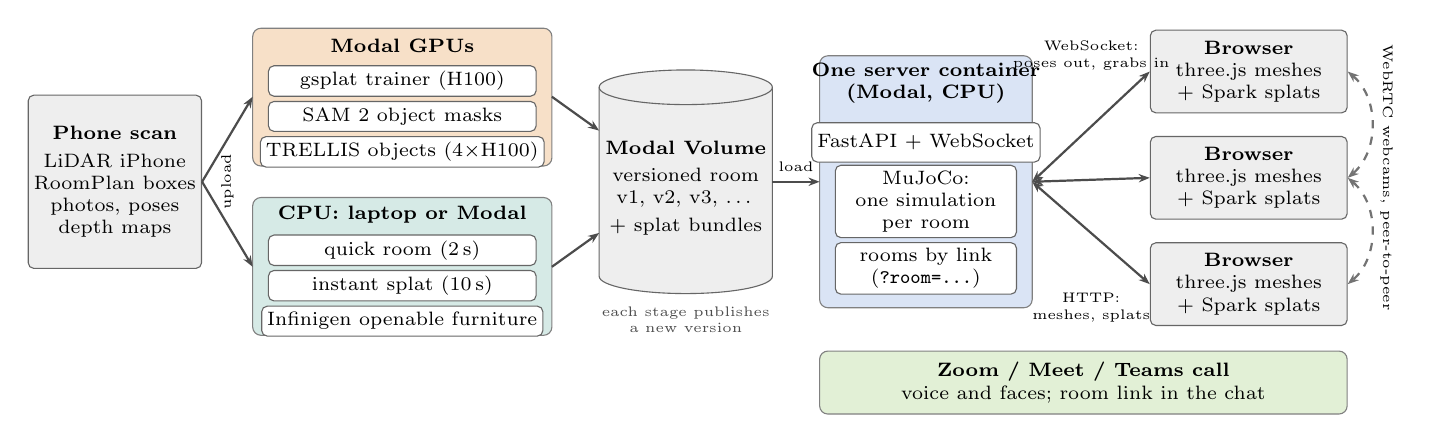
\begin{tikzpicture}[
    font=\scriptsize,
    >={Stealth[length=4pt]},
    flow/.style={->, thick, draw=black!70},
    box/.style={draw=black!60, rounded corners=2pt, align=center, inner sep=2pt},
    sub/.style={box, fill=white, minimum width=3.4cm, minimum height=0.38cm},
    ssub/.style={box, fill=white, minimum width=2.3cm, minimum height=0.5cm},
    group/.style={rounded corners=3pt, draw=black!50},
    title/.style={font=\scriptsize\bfseries, align=center},
    small/.style={font=\tiny, align=center},
  ]
  \definecolor{rcgpu}{RGB}{247,224,200}
  \definecolor{rccpu}{RGB}{214,234,230}
  \definecolor{rcsrv}{RGB}{218,228,245}
  \definecolor{rcweb}{RGB}{238,238,238}
  \definecolor{rcvc}{RGB}{226,240,214}

  % ---- 1. phone scan ------------------------------------------------------------------
  \node[box, fill=rcweb, minimum width=1.9cm, minimum height=2.2cm] (scan) at (0.95, 2.70)
    {\textbf{Phone scan}\\[2pt]LiDAR iPhone\\RoomPlan boxes\\photos, poses\\depth maps};

  % ---- 2. builders --------------------------------------------------------------------
  \draw[group, fill=rcgpu] (2.70, 2.90) rectangle (6.50, 4.65);
  \node[title] at (4.60, 4.43) {Modal GPUs};
  \node[sub] at (4.60, 3.98) {gsplat trainer (H100)};
  \node[sub] at (4.60, 3.53) {SAM~2 object masks};
  \node[sub] at (4.60, 3.08) {TRELLIS objects (4$\times$H100)};

  \draw[group, fill=rccpu] (2.70, 0.75) rectangle (6.50, 2.50);
  \node[title] at (4.60, 2.28) {CPU: laptop or Modal};
  \node[sub] at (4.60, 1.83) {quick room (2\,s)};
  \node[sub] at (4.60, 1.38) {instant splat (10\,s)};
  \node[sub] at (4.60, 0.93) {Infinigen openable furniture};

  \draw[flow] (scan.east) -- (2.70, 3.78);
  \draw[flow] (scan.east) -- (2.70, 1.62);
  \node[small, rotate=90] at (2.38, 2.70) {upload};

  % ---- 3. versioned room on a Modal Volume (cylinder drawn by hand) ---------------------
  \fill[rcweb] (7.10, 1.50) rectangle (9.30, 3.90);
  \fill[rcweb] (8.20, 1.50) ellipse [x radius=1.10, y radius=0.22];
  \draw[black!60] (7.10, 3.90) -- (7.10, 1.50)
        arc [start angle=180, end angle=360, x radius=1.10, y radius=0.22] -- (9.30, 3.90);
  \draw[black!60, fill=rcweb] (8.20, 3.90) ellipse [x radius=1.10, y radius=0.22];
  \node[align=center] at (8.20, 2.62)
    {\textbf{Modal Volume}\\[2pt]versioned room\\v1, v2, v3, \dots\\[2pt]+ splat bundles};
  \node[small, text=black!70] at (8.20, 0.95) {each stage publishes\\a new version};

  \draw[flow] (6.50, 3.78) -- (7.10, 3.35);
  \draw[flow] (6.50, 1.62) -- (7.10, 2.05);

  % ---- 4. one server container ----------------------------------------------------------
  \draw[group, fill=rcsrv] (9.90, 1.10) rectangle (12.60, 4.30);
  \node[title] at (11.25, 3.95) {One server container\\(Modal, CPU)};
  \node[ssub] at (11.25, 3.20) {FastAPI + WebSocket};
  \node[ssub] at (11.25, 2.45) {MuJoCo:\\one simulation\\per room};
  \node[ssub] at (11.25, 1.60) {rooms by link\\(\texttt{?room=\dots})};

  \draw[flow] (9.30, 2.70) -- node[above, small] {load} (9.90, 2.70);

  % ---- 5. browsers ----------------------------------------------------------------------
  \foreach \y/\n in {4.10/b1, 2.75/b2, 1.40/b3} {
    \node[box, fill=rcweb, minimum width=2.5cm, minimum height=1.05cm] (\n) at (15.35, \y)
      {\textbf{Browser}\\three.js meshes\\+ Spark splats};
  }
  \foreach \n in {b1, b2, b3} {
    \draw[<->, thick, draw=black!70] (12.60, 2.70) -- (\n.west);
  }
  \node[small] at (13.35, 4.30) {WebSocket:\\poses out, grabs in};
  \node[small] at (13.35, 1.10) {HTTP:\\meshes, splats};

  % WebRTC webcams go browser to browser, not through the server
  \draw[<->, dashed, thick, draw=black!55] (b1.east) to[bend left=50] (b2.east);
  \draw[<->, dashed, thick, draw=black!55] (b2.east) to[bend left=50] (b3.east);
  \node[small, rotate=-90] at (17.10, 2.75) {WebRTC webcams, peer-to-peer};

  % ---- the video call carries voice ------------------------------------------------------
  \draw[group, fill=rcvc] (9.90, -0.25) rectangle (16.60, 0.55);
  \node[align=center] at (13.25, 0.15)
    {\textbf{Zoom / Meet / Teams call}\\voice and faces; room link in the chat};
\end{tikzpicture}

  \caption{\sys{} architecture. A phone scan is uploaded to builders: Modal GPUs run the gsplat
  trainer, SAM~2 object masks and TRELLIS, and a CPU (the laptop or Modal) builds the quick room,
  the instant splat and Infinigen's openable furniture. Each stage publishes a new version of the
  room to a Modal Volume. One server container loads it and runs one MuJoCo simulation per room,
  sending body poses to every browser over a WebSocket and taking grabs back; rooms are created
  by link. Browsers draw meshes with three.js and splats with Spark. Webcams go browser to browser
  over WebRTC, and the video call carries voice as usual.}
  \Description{Block diagram, left to right: phone scan; builders split into a GPU group (gsplat
  trainer, SAM 2, TRELLIS) and a CPU group (quick room, instant splat, Infinigen); a Modal
  Volume holding versions of the room; one server container with FastAPI, WebSocket and MuJoCo;
  three browsers with two-way arrows to the server and dashed WebRTC links between them. A bar
  under the server and browsers stands for the Zoom, Meet or Teams call.}
  \label{fig:architecture}
\end{figure*}
Figure~\ref{fig:architecture} shows the system.

\paragraph{Server.} One CPU container holds every room. A room's simulation steps at real time
and broadcasts body poses. People grab with a spring to a hand target, and a throw keeps the
body's velocity. Rooms are created on demand by link (\texttt{?room=\dots}) and dropped when empty.

\paragraph{Versions.} Each build stage publishes a new version of the room. Browsers prefetch it
and swap at a frame boundary, and the server carries object positions and active grabs across by
body name. Splat bundles update on their own channel, since a training snapshot is not a new
physics version.

\paragraph{Clients.} three.js draws meshes and Spark~2.3 draws splats in the same scene. Each
movable object's splat is a child of its body's node. Picking uses the (hidden) collision meshes,
so grabbing the photoreal chair grabs the physical one. People appear as webcam holograms
(MediaPipe segmentation on the sender's device) or as full-body splat avatars (LHM++ on a GPU).

\section{From Scan to a Photoreal, Interactive Room}
\begin{table}[t]
\caption{Building the tea\_room scan (62 photos), measured from the start of each step. Costs are
Modal list prices.}
\label{tab:timeline}
\begin{tabular}{lrr}
\toprule
Stage & Ready at & Cost \\
\midrule
Quick room (RoomPlan boxes $\rightarrow$ templates, photo walls, physics) & \measured{2.0\,s} & \$0 \\
Instant splat (photos + LiDAR fused, no GPU) & \measured{10\,s} & \$0 \\
Objects cut out by SAM~2 masks (in parallel) & \measured{+15--18\,s} & \measured{$<$\$0.01} \\
Trainer up on an H100 (container warmed during the instant splat) & \measured{26\,s} & \\
First trained splat (step 400, 600k splats) & \measured{73\,s} & \\
Final trained splat (1250 steps $\times$ 4 photos, 800k splats) & \measured{104\,s} & \measured{$\approx$\$0.15} \\
Generated object meshes (TRELLIS, 4$\times$H100) & \measured{2.0--7.2\,min} & \measured{\$2.24} \\
Openable furniture (Infinigen-Sim, 7 assets, laptop CPU) & \measured{91\,s} & \$0 \\
\midrule
\multicolumn{3}{l}{\emph{Scanned during a call (deployed system, from the start of the upload):}} \\
Quick room in every browser & \measured{10\,s} & \\
Photoreal (instant splat, objects cut out) & \measured{22\,s} & \\
First trained snapshot & \measured{96\,s} & \\
\bottomrule
\end{tabular}
\end{table}
\begin{figure}[t]
  \centering
  % Progressive build of the tea_room scan as a horizontal timeline. One column wide (8.4 cm).
% Needs in the preamble:
%   \usepackage{tikz}
%   \usetikzlibrary{shapes.geometric}
% Time axis is logarithmic: x = 1.9 cm per decade, from 1 s (x = 0) to 10 min (x = 5.28).
% Numbers: paper Table "tab:timeline", results/tea_room/splat_run.md (trainer up 29.4 s,
% snapshots 81.3 / 112.8 / 141.9 s, final 184.3 s) and results/tea_room/realistic_run.md
% (TRELLIS first object 122 s, all previews 275 s, all finals 430 s). Openable furniture: 91 s.
% Every stage is timed from its own start; they all start when the scan arrives.
\begin{tikzpicture}[
    font=\scriptsize,
    x=1cm, y=1cm,
    lab/.style={anchor=east, align=right, font=\scriptsize},
    val/.style={font=\tiny, inner sep=1pt},
    ready/.style={draw=black, fill=#1, diamond, inner sep=0pt, minimum size=5pt},
    snap/.style={draw=black, fill=white, circle, inner sep=0pt, minimum size=3.5pt},
    bar/.style={line width=4pt, draw=#1},
    calld/.style={draw=black, fill=white, diamond, inner sep=0pt, minimum size=5pt},
  ]
  \definecolor{rccpu}{RGB}{56,140,128}
  \definecolor{rcgpu}{RGB}{214,120,40}
  \definecolor{rcgpulight}{RGB}{247,214,184}
  % \rctx{t}: x position of t seconds (an expression; TikZ evaluates it)
  \def\rctx#1{1.9*log10(#1)}

  % rows (y), top to bottom
  \def\yQ{5.0} \def\yI{4.3} \def\yT{3.6} \def\yF{2.9} \def\yO{2.2} \def\yC{1.3}

  % grid and axis
  \foreach \t in {1, 2, 5, 10, 30, 60, 120, 300, 600} {
    \draw[black!12] (\rctx{\t}, 0.85) -- (\rctx{\t}, 5.35);
  }
  \draw[->, black!70] (0, 0.85) -- (5.45, 0.85);
  \foreach \t/\l in {1/1\,s, 2/2\,s, 5/5\,s, 10/10\,s, 30/30\,s, 60/1\,min, 120/2\,min, 300/5\,min, 600/10\,min} {
    \draw[black!70] (\rctx{\t}, 0.85) -- (\rctx{\t}, 0.78);
    \node[font=\tiny, anchor=north, inner sep=1pt] at (\rctx{\t}, 0.77) {\l};
  }
  \node[font=\tiny, anchor=north] at (2.7, 0.42) {time since the scan arrived (log scale)};

  % row labels
  \node[lab] at (-0.12, \yQ) {Quick room};
  \node[lab] at (-0.12, \yI) {Instant splat};
  \node[lab] at (-0.12, \yT) {Trained splat\\[-1pt]\tiny gsplat, 1$\times$H100};
  \node[lab] at (-0.12, \yF) {Openable furniture\\[-1pt]\tiny Infinigen, CPU};
  \node[lab] at (-0.12, \yO) {Object meshes\\[-1pt]\tiny TRELLIS, 4$\times$H100};
  \node[lab] at (-0.12, \yC) {In a live call\\[-1pt]\tiny deployed, from upload};
  \draw[black!30] (-2.3, 1.75) -- (5.45, 1.75);

  % quick room: 2.0 s (CPU)
  \node[ready=rccpu] at (\rctx{2}, \yQ) {};
  \node[val, anchor=west] at ({\rctx{2}+0.08}, \yQ) {2\,s};

  % instant splat: 10 s (CPU)
  \node[ready=rccpu] at (\rctx{10}, \yI) {};
  \node[val, anchor=west] at ({\rctx{10}+0.08}, \yI) {10\,s, photoreal};

  % trained splat: trainer up at 29.4 s, first snapshot 81-102 s, final 184 s
  \draw[bar=rcgpulight] (\rctx{29.4}, \yT) -- (\rctx{81.3}, \yT);
  \draw[bar=rcgpu] (\rctx{81.3}, \yT) -- (\rctx{184.3}, \yT);
  \foreach \t in {112.8, 141.9} { \node[snap] at (\rctx{\t}, \yT) {}; }
  \node[ready=rcgpu] at (\rctx{81.3}, \yT) {};
  \node[ready=rcgpu] at (\rctx{184.3}, \yT) {};
  \node[val, anchor=south] at (\rctx{81.3}, {\yT+0.1}) {first 81--102\,s};
  \node[val, anchor=west] at ({\rctx{184.3}+0.08}, \yT) {final 184\,s};
  \node[val, anchor=north, text=black!60] at ({0.5*(\rctx{29.4}+\rctx{81.3})}, {\yT-0.08}) {training};

  % openable furniture: 91 s (CPU)
  \node[ready=rccpu] at (\rctx{91}, \yF) {};
  \node[val, anchor=west] at ({\rctx{91}+0.08}, \yF) {91\,s};

  % TRELLIS objects: first at 122 s, all previews 275 s, all finals 430 s
  \draw[bar=rcgpu] (\rctx{122}, \yO) -- (\rctx{430}, \yO);
  \node[ready=rcgpu] at (\rctx{122}, \yO) {};
  \node[snap] at (\rctx{275}, \yO) {};
  \node[ready=rcgpu] at (\rctx{430}, \yO) {};
  \node[val, anchor=east] at ({\rctx{122}-0.1}, \yO) {2.0--7.2\,min};

  % the deployed system in a call: quick room 10 s, photoreal 22 s, first trained snapshot 96 s
  \foreach \t/\l in {10/10\,s, 22/22\,s, 96/96\,s} {
    \node[calld] at (\rctx{\t}, \yC) {};
    \node[val, anchor=south] at (\rctx{\t}, {\yC+0.1}) {\l};
  }
  \node[val, anchor=north east] at ({\rctx{10}+0.1}, {\yC-0.1}) {mesh room};
  \node[val, anchor=north west] at ({\rctx{22}-0.1}, {\yC-0.1}) {photoreal};
  \node[val, anchor=north, align=center] at (\rctx{96}, {\yC-0.1}) {trained};

  % legend
  \node[ready=rccpu] at (0.05, 5.65) {};
  \node[val, anchor=west] at (0.15, 5.65) {CPU stage ready};
  \node[ready=rcgpu] at (1.75, 5.65) {};
  \node[val, anchor=west] at (1.85, 5.65) {GPU stage ready};
  \node[snap] at (3.45, 5.65) {};
  \node[val, anchor=west] at (3.55, 5.65) {intermediate};
\end{tikzpicture}

  \caption{Progressive build of tea\_room (62 photos), on a log time axis. Each stage is timed
  from its own start; all start when the scan arrives and run in parallel. The trained splat
  streams snapshots from step 400 (73\,s) to the final splat at 104\,s, uploads to the deployed link included; generated objects
  arrive one at a time between 2.0 and 7.2\,min (circle: all previews, 275\,s). Bottom row: the
  deployed system when a room is scanned during a call, timed from the start of the upload.}
  \Description{Horizontal timeline with a logarithmic time axis from 1 second to 10 minutes.
  Quick room ready at 2 seconds; instant splat at 10 seconds; trained splat training from
  26 seconds, first snapshot at 73 seconds and final at 104 seconds; openable furniture at
  91 seconds; generated object meshes from 2.0 to 7.2 minutes. A separate row for a live call
  marks the mesh room at 10 seconds, the photoreal room at 22 seconds and the first trained
  snapshot at 96 seconds.}
  \label{fig:timeline}
\end{figure}

\paragraph{Instant splat.} Every LiDAR depth sample of every photo becomes a flat disc, oriented
along the surface normal and sized to the surface patch the pixel covers. Discs are fused on a
voxel grid: per voxel, the sharpest view's geometry and the confidence-weighted mean colour.
\measured{640k} splats, \measured{6\,MB}, \measured{10\,s} on a laptop CPU.

\paragraph{Trained splat.} gsplat's trainer runs unchanged on a training set written directly
from the scan. ARKit poses and intrinsics are the cameras, so no COLMAP is needed. Confident LiDAR
samples initialise the splats and supervise depth, and a per-photo bilateral grid absorbs the
phone's exposure changes. The H100 is bound by per-step overhead rather than pixels, so we train on
four photos per step for 1250 steps with fused bilateral-grid and visible-splat Adam kernels: the
training loop takes \measured{33\,s} and the held-out PSNR rises from \measured{19.17} to
\measured{20.2\,dB} against a 7000-step single-photo schedule
(\texttt{results/tea\_room/splat\_speed.md}). A warm-up call boots the GPU container while the
instant splat is computed. Snapshots stream to the call as they are produced.

\paragraph{Interactive objects.} For each movable body:
\begin{enumerate}
  \item The body's box is projected into the photos that see it best, grown by 30\% because
        RoomPlan places chairs 20--30\,cm off.
  \item SAM~2 returns three candidate masks per box. We keep the best-scoring one that is not
        mostly static furniture, judged by lifting its pixels with LiDAR depth, so a chair tucked
        under a table is not mistaken for the table.
  \item Every splat near the body votes, by projection into those photos with a LiDAR
        visibility test. A splat inside the mask in at least two photos and half of the photos
        that saw it belongs to the object.
  \item The body is then moved to the median of its splats, measured on the instant splat whose
        splats lie on surfaces. The move is scaled back if it would push the body deeper into
        walls or static furniture than its scanned pose.
  \item The floor under each object, never photographed, is patched with splats coloured from the
        surrounding floor.
\end{enumerate}

\section{Evaluation}
\subsection{Visual fidelity}
We render each stage as the call draws it (headless Chromium, software WebGL), from every photo's
own camera, and compare at 320$\times$240 (Table~\ref{tab:fidelity}). Object pixels come from
LiDAR depth inside RoomPlan boxes. The splat is also scored separately on the trainer's held-out
photos.
\begin{table}[t]
\caption{Fidelity against the scan's own photos (tea\_room, 16 views at 320$\times$240, rendered
as the call draws them in headless software WebGL). Differences are paired over views, with 95\%
percentile-bootstrap intervals (10{,}000 resamples).}
\label{tab:fidelity}
\begin{tabular}{lrrrr}
\toprule
Stage & PSNR & SSIM & PSNR walls/floor & PSNR objects \\
\midrule
Flat mean colour (baseline) & \measured{13.75} & & & \\
Mesh room: photo walls + TRELLIS objects & \measured{13.64} & \measured{0.679} & \measured{14.40} & \measured{11.54} \\
Trained splat (objects cut out) & \measured{18.47} & \measured{0.788} & \measured{18.72} & \measured{19.11} \\
\midrule
Splat $-$ mesh & \measured{+4.83} [2.74, 6.67] & \measured{+0.108} & \measured{+4.31} & \measured{+7.57} [5.66, 9.74] \\
\bottomrule
\end{tabular}
\end{table}
On the four views the splat trainer held out, the splat scores \measured{17.45\,dB} against
\measured{11.66\,dB} for the mesh room on its two unseen views. The gain is largest on objects,
where the mesh room shows generated meshes and the splat shows the photographed objects
themselves. With the photo-corrected body poses, all \measured{5/5} movable bodies in the splat
room's physics are interactable, against \measured{3/5} at RoomPlan's poses: two chairs RoomPlan
had boxed into the table become free once moved to where the photos show them.

\subsection{Physics and capacity}
Every movable part is grabbed and pulled through the server's own simulation, then released
(the audit of \texttt{litereality evaluate}). With Infinigen's openable furniture, tea\_room has
17 moving parts:
\begin{itemize}
  \item \textbf{Interactable} (grabbed, moved by the pull, at rest after release):
        \measured{12/17}. That is \measured{8/9} hinges and both window sashes.
  \item \textbf{Failures:} two chairs tucked under the table, which the pull cannot free; and
        the dishwasher. Its door's holding friction is sized for the door lying flat, so a pull
        cannot open it from closed, and its racks cannot slide while the door is shut.
  \item \textbf{Masses:} \measured{2/17} fall outside per-category plausible ranges (window
        sashes slightly light).
  \item \textbf{Stability:} no interpenetration above 5\,mm and no drift over 10\,s.
  \item \textbf{Cost:} a step costs \measured{0.18--0.25\,ms}, so one room runs
        \measured{8--11$\times$} faster than real time on one thread. One server process held
        \measured{16} rooms (its cap) in real time.
\end{itemize}

\subsection{Estimated physics}
\todo{physics study: LiteReality vs an LLM vs measured mass, friction, restitution
(doc/physics\_study.md)}.

\section{User Study}
\todo{protocol in paper/study\_protocol.md: 12--16 pairs; video vs mesh room vs photoreal room;
spatial Q\&A, rearrangement, hand-over; IPQ, co-presence, NASA-TLX, logs, interviews.}

\section{Limitations}
Objects tucked deep under other furniture are seen too little to be segmented reliably (one of
four chairs in tea\_room). Splats behind a moved object are missing, and only the floor is
patched. View-dependent highlights on moved objects are not re-lit. MuJoCo ignores restitution.
Webcam video is peer-to-peer without a TURN relay. Physics is estimated, not measured, unless the
physics study's measurements are loaded.

\bibliographystyle{ACM-Reference-Format}
\bibliography{refs}
\end{document}
